\section{Analisi della rete}\label{misuregenerali}

    La nostra rete è composta da $N = 16675$ nodi e $L = 52373$ collegamenti.
    
    \subsection{Misure generali e di connessione}
    
    \subsubsection{Distribuzione dei gradi dei nodi}
        
        \begin{figure}[ht]
            \centering
            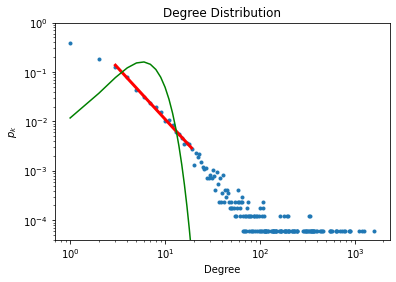
\includegraphics[width=6.5cm]{3_analysis_network/degree.png}
            \caption{Grafico in scala bilogaritmica. In blu: distribuzione del grado dei nodi. In rosso: fit in regime di legge a potenza. In verde: forma della distribuzione di Poissont con $\left<k\right>=\frac{2L}{N}\simeq6.28$.}
            \label{Degree_distribution}
        \end{figure}
        
        In figura \ref{Degree_distribution} mostriamo la distribuzione del grado dei nodi in confronto ad una distribuzione poissoniana. La nostra rete ha un comportamento molto diverso rispetto a quest'ultima, in particolare sulle code.
        Nonostante il grado medio dei nodi della rete sia $\left< k \right> \simeq 6.28$, circa il 60\% dei nodi ha avuto solo una o due interazioni, mentre ce ne sono altri, i cosiddetti \textit{hubs}, che ne hanno oltre $10^2-10^3$ (figura \ref{Degree_distribution}). Una distribuzione di questo tipo viene detta a \textit{fat tail}, tipica delle reti reali \cite{barabasicap3}.
        
        Il grafico bilogaritmico suggerisce una descrizione della distribuzione tramite una legge a potenza del tipo $p(k)=Ck^{-\gamma}$ e, tramite un fit nella regione in cui tale comportamento è più evidente, abbiamo ottenuto $\gamma=2.09 \pm 0.04$ che, essendo $2 \leq \gamma \leq 3$, colloca la nostra rete nel regime di invarianza di scala.

        \subsubsection{Coefficiente di clustering e densità}
        Il coefficiente di clustering medio della nostra rete è stato calcolato con la media dei coefficienti di clustering locali di tutti i nodi della rete:
        \begin{equation}
            \left< C_i \right> = \left< \frac{2e_i}{k_i(k_i-1)} \right>=0.274,
            \label{clustering_coefficient}
        \end{equation}
        dove $e_i$ sono le connessioni fra i vicini del nodo $i$. Il valore è abbastanza alto da poter essere considerato in linea con i valori attesi per le \textit{real-word social network} \cite{barabasicap3}.
        
        La densità di un grafo, definita dal rapporto tra i link esistenti e tutti i link possibili all’interno del grafo stesso, nella nostra rete è 
        \begin{equation}
            d =\frac{L}{L_{max}}=\frac{2L}{N(N-1)}=0.00038,
            \label{densità}
        \end{equation}
        un valore molto piccolo ($d<<1$), come ci si aspetta in reti sparse, ovvero debolmente connesse, tipicamente osservate in sistemi reali, come la nostra, dove $L << L_{max}$ $\simeq 1,4\times10^8$ \cite{barabasicap2}. 
    
    \subsubsection{Cammini e distanze}              
    Dopo aver estratto la \textit{giant component}, ovvero la componente connessa più grande, abbiamo calcolato la lunghezza media del cammino più breve ($\left< d \right> = 3.94$) e il diametro ($d_{max}$ = 12). 
        
    Rispetto alla rete totale, la densità aumenta leggermente ($d_{gc}=0.0004$), mentre il coefficiente di clustering medio resta pressoché invariato ($\left< C_{gc}\right>=0.278$). 
    Sebbene nella nostra rete siano presenti 230 componenti connesse, questa evidente somiglianza dei valori è dovuta al fatto che la maggior parte dei nodi ($N_{gc}=16074$) appartengano alla \textit{giant component}, che costituisce circa il $96.4\%$ del grafo totale. Il numero di edges della \textit{giant component} è $L_{gc}=51932$.
    
\subsection{Confronto con reti sintetiche}

    \begin{table*}[pb]
        \centering
        \small
        \rowcolors{1}{}{lightgray}
        \begin{tabular}{|c|rrrrrr|} 
            \hline
             & Nodi & Links & $\left<k\right>$ & $\,d$ & $\left<C\right>$ & $d_{max}$ \\ 
            \hline
            Rete reale & 16675 & 52373 & 6.28 & 0.00038 & 0.27 & 12 \\
            Erdos-Renyi & 16675 & 52074 & 6.25 & 0.00037 & 0.0004 & 10 \\
            Watts-Strogatz & 16675 & 50025 & 6.0 & 0.00036 & 0.44 & 16 \\
            Barabasi-Albert & 16675 & 50016 & 6.0 & 0.00036 & 0.0034 & 7 \\
            Configuration model & 16675 & 52373 & 6.28 & 0.00038 & 0.34 & 9 \\
            \hline
        \end{tabular}
        \caption{Informazioni delle varie reti. $\left<k\right>$: grado medio; $d$: densità; $\left<C\right>$: coefficiente di cluster medio; $d_{max}$: diametro.}
        \label{table: networks_comparison}
    \end{table*}

    In tabella \ref{table: networks_comparison}, riportiamo alcune misure statistiche effettuate sulla nostra rete comparate con quelle ottenute su versioni random della stessa generate da diversi modelli. 
    
    \paragraph{\tab Confronto con il modello Erdos-Rényi.} Per costruire un grafo Erdos-Renyi che avesse lo stesso numero di nodi e (approssimativamente) di collegamenti della nostra rete abbiamo utilizzato $N$ e abbiamo collegato ogni coppia con probabilità

            \begin{equation}
                p = \frac{\left<k\right>}{N-1} = 0.00038
            \end{equation}
    al fine di ottenere un valore atteso $E(L_{er})$ della rete sintetica uguale a quello della nostra rete.
        
    Il grafo ottenuto ha 16675 nodi, 52074 links ed è composto da 36 componenti connesse. Si noti che il coefficiente di clustering medio è di diversi ordini di grandezza più basso ($\left< C_i \right> =0.00037$), come è previsto per le reti random \cite{barabasicap3}. 
        
    La distribuzione dei nodi è binomiale (figura \ref{Random_model_distribution}) e non rispecchia la distribuzione a coda lunga, caratteristica delle reti reali e riscontrata nella nostra rete (figura \ref{Degree_distribution}).
    La rete ha un grande numero di nodi con un grado $\left<k_{er}\right> \simeq 6.25$, e pochi nodi con un grado che si discosta molto da tale media. 
    
     \begin{figure}[ht]
            \centering
            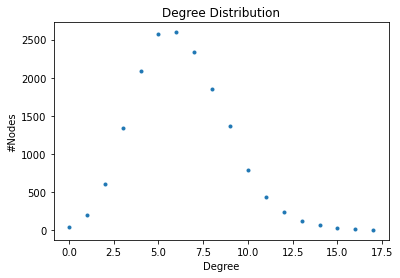
\includegraphics[width=7cm] {3_analysis_network/poissont.png}
            \caption{Grado vs numero di nodi aventi quel determinato grado nella rete random.}
            \label{Random_model_distribution}
        \end{figure}
    
     \paragraph{\tab Confronto con il modello Watts-Strogatz.}
     Per costruire un grafo Watts-Strogatz che avesse lo stesso numero di nodi e (approssimativamente) di collegamenti della nostra rete abbiamo utilizzato $N$, impostato il numero di vicini a 6 e la \textit{rewiring probability} $p_{ws} = 0.1$, così da ottenere $N_{ws}=16675$ e $L_{ws}=50025$ con un grado medio $k_{ws} = 6$, uguale appunto al vicinato impostato. Il coefficiente di clustering medio è 0.44.
    
     \paragraph{\tab Confronto con il modello Barabasi-Albert.} Abbiamo implementato una rete con il modello Barabasi-Albert avente 16675 nodi e 50016 links. Per ottenere un numero di collegamenti quanto più vicino a $L$, abbiamo impostato il parametro $m$, ovvero il numero di vicini a cui collegare un nuovo nodo, a 3. La rete è composta da un’unica componente connessa. Il grado medio è 6.0, abbastanza simile a quello della nostra rete, mentre il coefficiente di clustering medio risulta essere significativamente minore (0.003 \textit{vs} 0.27). La densità è 0.00036, conforme a quella della nostra rete.
    
     \paragraph{\tab Confronto con il Configuration model.}
     Abbiamo creato un Configuration model con 16675 nodi e 52373 link, composto da 194 componenti connesse. Come vediamo in tabella \ref{table: networks_comparison} i valori di questo modello sono i più vicini a quelli della nostra rete. In questo caso, si ottiene un multigrafo, un tipo di rete non supportato dalla funzione di \textit{average clustering} della libreria Networkx. Abbiamo dunque utilizzato la formula \cite{barabasicap7}
        
        \begin{equation}
            C_{cm}=\frac{\left( \left<k^2\right>-\left<k\right>\right)^2}{N \left<k\right>^3}.
            \label{clustering_configuration}
        \end{equation}
        
    \begin{figure*}[b]
        \centering
        \begin{subfigure}{.4\textwidth}
            \centering
            \caption{}
            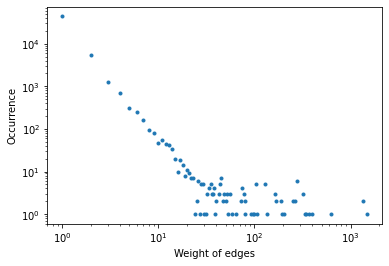
\includegraphics[scale=.4]{6_Network_resilience/equal_weights.png}
            \label{fig:equal_weights}
        \end{subfigure}
        \centering
        %\vspace{-3mm}
        \begin{subfigure}{.4\textwidth}
            \centering
            \caption{}
            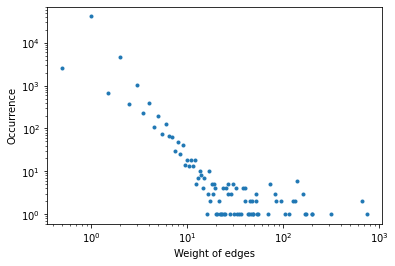
\includegraphics[scale=.4] {6_Network_resilience/direct_undirect_weights.png}
            \label{fig:direct_undirect_weights}
        \end{subfigure}
        \caption{Distribuzione delle occorrenze dei pesi con \textit{links} di peso unitario (\subref{fig:equal_weights}) e \textit{links} di primo e di secondo livello (\subref{fig:direct_undirect_weights})}
        \label{fig:weights}
    \end{figure*}

    \subsection{Misure di centralità}
    
        \begin{table*}
        \centering
        %\small
        \caption{Nodi con il punteggio più alto per varie centralità.}
        \resizebox{\textwidth}{!}{%
            \begin{tabular}{|cl|cl|cl|cl|} 
                \hline
                \multicolumn{2}{|c|}{\textbf{Eigenvector centrality}} & \multicolumn{2}{c|}{\textbf{Closeness centrality}} & \multicolumn{2}{c|}{\textbf{Betweeness centrality}} & \multicolumn{2}{c|}{\textbf{Harmonic centrality}} \\ 
                \hline
                repubblica~ & 0.337 & JFSebastian146 & 0.401 & JFSebastian146 & 0.106 & JFSebastian146 & 0.433 \\
                PBerizzi~ & 0.281 & repubblica~ & 0.371 & repubblica~ & 0.080 & repubblica~ & 0.423 \\
                feltrinellied~ & 0.262 & Vivo\_Azzurro & 0.371 & Giorgiolaporta~ & 0.075 & PBerizzi~ & 0.412 \\
                fratolo2~ & 0.147 & Azzurri~ & 0.368 & lefrasidiosho~ & 0.072 & fratotolo2~ & 0.406 \\
                Vivo\_Azzurro & 0.134 & Azzurri\_Ar~ & 0.368 & PBerizzi~ & 0.057 & Vivo\_Azzurro~ & 0.405 \\
                \hline
            \end{tabular}
         }
        \label{table: Centrality}
    \end{table*}
        
        Le misure di centralità definite sulla topologia della rete sono dei valori che definiscono l’"importanza" di un nodo sulla base di come esso è disposto nel grafo o connesso ad altri nodi. 
        
        In tabella \ref{table: Centrality} sono riportati i primi cinque nodi per diversi tipi di centralità. @repubblica, @JFSebastian146, @PBerizzi e @Vivo\_Azzurro (pagina ufficiale della Nazionale di calcio) sono presenti nella top 5 di ben 3 misure su 4. Nello specifico, si nota come l'utente @JFSebastian146 figuri al primo posto in ogni misura di centralità geometrica (centralità di \textit{closeness}, \textit{betweeness} e \textit{harmonic}) mentre non compaia affatto nella classifica relativa all'\textit{Eigenvector centrality}. Tale nodo occupa, dunque, una posizione centrale dal punto di vista topologico, ovvero è mediamente più vicino a tutti gli altri nodi della rete e attraversato da molti \textit{shortest path}, senza però essere collegato ad altri nodi rilevanti del grafo.
        
        Non banale è il fatto che solo 4 dei 10 differenti utenti che compaiono nelle classifiche proposte siano effettivamente autori di tweet e non utenti menzionati tramite tag. Si tratta di account piuttosto seguiti - @lefrasidiosho (450075 followers, 1 tweet pubblicato), @Giorgiolaporta (58129 followers, 3 tweets) e @PBerizzi (29174 followers, 3 tweets) - ad eccezione di @JFSebastian146, che supera di poco gli 8mila followers, a fronte però di un elevatissimo numero di tweet e  retweet: ben 454. Si rimanda al paragrafo \ref{who} per ulteriori approfondimenti. 
   
    
    \section{Resilienza della rete}\label{netres}
    
    Analizziamo ora l'impatto dei legami forti e deboli sulla connettività e sulla resilienza della rete.
        
    \subsection{Definizione dei pesi}
    
    Come accennato in sezione \ref{costruzionerete}, nella nostra rete, la connessione degli utenti di Twitter può avvenire sostanzialmente in due modi: 
        \begin{enumerate}\label{interazione}
            \item interazioni attive, o di primo livello:
            \begin{enumerate}
                \item tra l'utente (attributo \texttt{user}) e l'autore del tweet al quale risponde (attributo \texttt{reply\_to}), che condivide (\texttt{retweets}), o che cita\footnote{Dal \href{https://help.twitter.com/it/resources/glossary}{Glossario} di Twitter: Cita tweet. Prima di ritwittare ai tuoi follower il Tweet di un altro utente, hai la possibilità di aggiungervi commenti, foto o una GIF.} (\texttt{quote\_to});
                \item tra l'autore del tweet (\texttt{user}) e ogni utente menzionato (\texttt{mentions}) nel tweet;
            \end{enumerate}
            \item interazioni passive, o di secondo livello:
             \begin{enumerate} 
                \item tra l'utente che ritwitta, cita o risponde ad un tweet e l'utente (o eventualmente più di uno) menzionato nel tweet. 
             \end{enumerate}
        \end{enumerate}
    
    Una prima maniera di attribuire un peso a questi legami potrebbe essere semplicemente quella di assegnare un valore unitario a qualsiasi tipo di interazione e successivamente contare il numero di interazioni fra due utenti. In questo modo, come è mostrato in figura \ref{fig:equal_weights}, la distribuzione delle occorrenze dei pesi è in scala bilogaritmica e segue una legge a potenza.

    Ciò nonostante, una comune assegnazione del peso a così diversi tipi di collegamenti ci è sembrata troppo sommaria e abbiamo preferito optare per una distizione fra i due tipi di connessioni, assegnando peso unitario ($w_{p} = 1$) alle interazioni \textit{di primo livello} e la metà ($w_{s} = 0.5$) a quelle \textit{di secondo livello}. Il peso finale $w_{uv}$ di un \textit{edge} tra il nodo \textit{u} e il nodo \textit{v} è dato dalla somma dei pesi di ogni interazione avvenuta tra i due nodi.  
    
    La figura \ref{fig:direct_undirect_weights} mostra la nuova distribuzione delle occorrenze dei pesi. Qualitativamente, si intravede ancora un andamento a potenza, sebbene i primi valori tendano a discostarsi. Il numero delle connessioni di secondo livello che abbiamo considerato è, infatti, molto minore rispetto alle altre. Ciò fa sì che si venga a creare una doppia retta nei primi valori, che solo successivamente arrivano a convergere.

    \subsection{Risultati}
    
    Per analizzare l’impatto della forza dei legami sulla connettività e sulla resilienza della rete, abbiamo proceduto a romperli in maniera ordinata, sia in senso crescente (dal meno forte al più forte) che decrescente, monitorando il progressivo cambiamento nelle dimensioni della \textit{giant component} (fig. \ref{fig:increasing_edges_removal} e \ref{fig:decreasing_edges_removal}).
    
    \begin{figure*}[ht]
        \centering
        \begin{subfigure}{.3\textwidth}
            \caption{}
            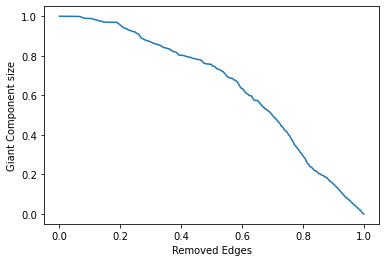
\includegraphics[scale=.34]{6_Network_resilience/increasing_edges_removal.png}
            \label{fig:increasing_edges_removal}
        \end{subfigure}
        \centering
        %\vspace{-3mm}
        \begin{subfigure}{.3\textwidth}
            \caption{}
            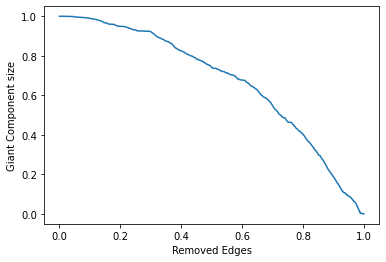
\includegraphics[scale=.34]{6_Network_resilience/decreasing_edges_removal.png}
            \label{fig:decreasing_edges_removal}
        \end{subfigure}
        \centering
        \begin{subfigure}{.3\textwidth}
            \caption{}
            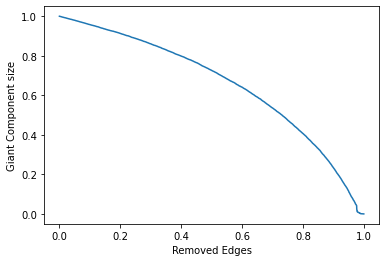
\includegraphics[scale=.34]{6_Network_resilience/random_edges_removal.png}
            \label{fig:random_edges_removal}
        \end{subfigure}
        \vspace{-3mm}
        \caption{Giant component size vs percentuale degli edges rimossi in ordine crescente (a), in ordine decrescente (b), in ordine random (c)}
        \label{fig:removal_edge}
    \end{figure*}
    
    Entrambi i grafici hanno un andamento simile a quello in figura \ref{fig:random_edges_removal}, in cui è rappresentato l'andamento della rete in relazione alla percentuale di \textit{edges} rimossi in maniera randomica. Guardando più nel dettaglio la figura \ref{fig:increasing_edges_removal}, è possibile notare una caduta leggermente più brusca quando si arriva ad eliminare circa il 20\% degli \textit{edges} più pesanti, che però potrebbe non essere abbastanza da suggerire una particolare importanza di questa fascia di \textit{edges} per la connettività della rete.
    
    La figura \ref{fig:random_edges_removal} ci mostra un comportamento tipico di una transizione di fase, con punto di transizione di qualche unità percentuali degli edges. Provando a fittare l'andamento con una funzione della forma $f(x)=(1-\frac{x}{x_c})^\beta$, dove $x$ è la percentuale di link rimossi, abbiamo ottenuto $\beta\simeq0.46$ e un punto di transizione (critico) $x_c\simeq 0.95$, mentre il punto di transizione teorico, ottenibile ponendo $\left<k\right>=1$, è $x_c=1-\frac{N}{2L}\simeq 0.84$.
    
    \begin{figure}
        \begin{subfigure}{.5\textwidth}
            \centering
            \caption{}
            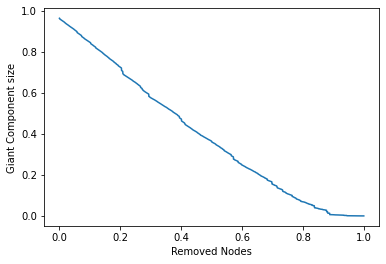
\includegraphics[scale=.4]{6_Network_resilience/random_node_dismantle.png}
            \label{fig:Random_network_resilience}
        \end{subfigure}
        \centering
        %\vspace{-3mm}
        \begin{subfigure}{.5\textwidth}
            \centering
            \caption{}
            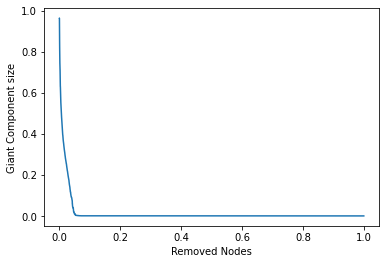
\includegraphics[scale=.4]{6_Network_resilience/hubs_node_dismantle.png}
            \label{fig:Hubs_network_resilience}
        \end{subfigure}
        \caption{Dimensione della giant component \textit{vs} percentuale dei nodi rimossi in maniera randomica (\subref{fig:Random_network_resilience}) e in ordine decrescente secondo la \textit{degree centrality} (\subref{fig:Hubs_network_resilience})}
        \label{fig:weights_1}
    \end{figure}
    
    Infine è stata analizzata la resilienza della rete rispetto all’eliminazione dei nodi, ordinati per ordine di grado (dal maggiore al minore). Risulta evidente che gli \textit{hubs} siano estremamente importanti ai fini della "conversazione" e già rimuovendo circa il primo 5\% la dimensione della \textit{giant component} diventi praticamente zero. Al contrario, quando i nodi vengono rimossi randomicamente (figura \ref{fig:Random_network_resilience}) le dimensioni della \textit{giant component} decadono linearmente con la percentuale di nodi rimossi, mostrando come la rete sia molto più resistente.
    
    




    